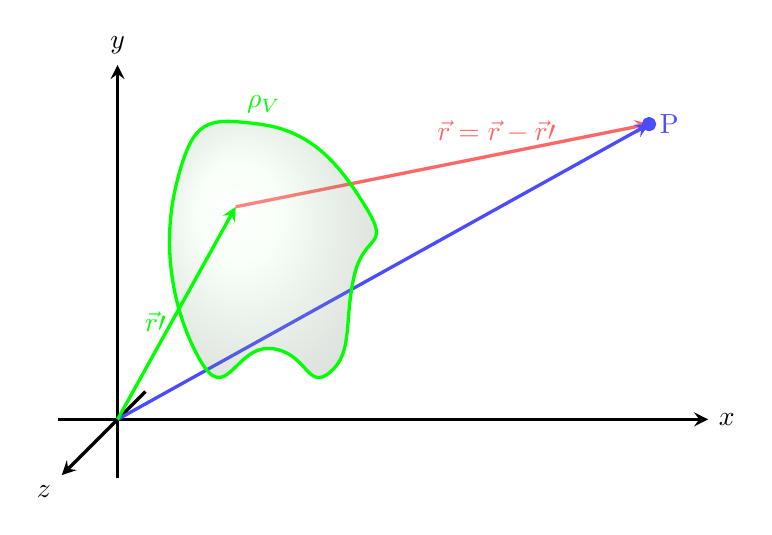
\begin{tikzpicture}[line width = 1.2pt, line join=round,x=1.5cm,y=1.5cm,z={(-0.35355cm,-0.35355cm)},>=stealth]
	% Koordinatensystem
	\draw [->] (-0.5,0) -- (5,0) node[anchor=west] {$x$};
	\draw [->] (0,-0.5) -- (0,3) node[anchor=south] {$y$};
	\draw [->] (0,0,-1) -- (0,0,2) node[anchor=north east] {$z$};
	% Differenzvektor R
	\draw [->, color=red!60] (1,1.8) -- (4.5,2.5);
	\draw [color=red!60] (3.8,2.25) node[anchor=south east] {$\vec{r}  = \vec{r}  - \vec{r}\prime  $};
	% Aufpunkt
	\draw [->,color=blue!70] (0,0) -- (4.5,2.5) node[anchor=west] {$\mathrm{P} $};
	\filldraw [color=blue!70] (4.5,2.5) circle (2pt);
	% Ladungsdichte
	\coordinate (a) at (2.1,1.8);
	\coordinate (b) at (2,1.2);
	\coordinate (c) at (1.8,0.4);
	\coordinate (d) at (1.3,0.6);
	\coordinate (e) at (0.7,0.5);
	\coordinate (f) at (0.5,2);
	\coordinate (g) at (1.2,2.5);
	\shade[ball color=white!10!green!20,opacity=0.20] plot [smooth cycle, tension = 1] coordinates {(a) (b) (c) (d) (e) (f) (g)};
	\draw [color=green] plot [smooth cycle, tension = 1] coordinates {(a) (b) (c) (d) (e) (f) (g)} node [sloped, above] {\ $ \rho_\text{V} $};
	\draw [->,color=green] (0,0) -- (1,1.8);
	\draw [color=green] (0.5,1.0) node[anchor=north east] {$ \vec{r}\prime  $};
\end{tikzpicture}